% mnras_template.tex 
%
% LaTeX template for creating an MNRAS paper
%
% v3.3 released April 2024
% (version numbers match those of mnras.cls)
%
% Copyright (C) Royal Astronomical Society 2015
% Authors:
% Keith T. Smith (Royal Astronomical Society)

% Change log
%
% v3.3 April 2024
%   Updated \pubyear to print the current year automatically
% v3.2 July 2023
%	Updated guidance on use of amssymb package
% v3.0 May 2015
%    Renamed to match the new package name
%    Version number matches mnras.cls
%    A few minor tweaks to wording
% v1.0 September 2013
%    Beta testing only - never publicly released
%    First version: a simple (ish) template for creating an MNRAS paper

%%%%%%%%%%%%%%%%%%%%%%%%%%%%%%%%%%%%%%%%%%%%%%%%%%
% Basic setup. Most papers should leave these options alone.
\documentclass[fleqn,usenatbib]{mnras}

% MNRAS is set in Times font. If you don't have this installed (most LaTeX
% installations will be fine) or prefer the old Computer Modern fonts, comment
% out the following line
\usepackage{newtxtext,newtxmath}
% Depending on your LaTeX fonts installation, you might get better results with one of these:
%\usepackage{mathptmx}
%\usepackage{txfonts}

% Use vector fonts, so it zooms properly in on-screen viewing software
% Don't change these lines unless you know what you are doing
\usepackage[T1]{fontenc}

% Allow "Thomas van Noord" and "Simon de Laguarde" and alike to be sorted by "N" and "L" etc. in the bibliography.
% Write the name in the bibliography as "\VAN{Noord}{Van}{van} Noord, Thomas"
\DeclareRobustCommand{\VAN}[3]{#2}
\let\VANthebibliography\thebibliography
\def\thebibliography{\DeclareRobustCommand{\VAN}[3]{##3}\VANthebibliography}


%%%%% AUTHORS - PLACE YOUR OWN PACKAGES HERE %%%%%

% Only include extra packages if you really need them. Avoid using amssymb if newtxmath is enabled, as these packages can cause conflicts. newtxmatch covers the same math symbols while producing a consistent Times New Roman font. Common packages are:
\usepackage{graphicx}	% Including figure files
\usepackage{amsmath}	% Advanced maths commands

%%%%%%%%%%%%%%%%%%%%%%%%%%%%%%%%%%%%%%%%%%%%%%%%%%

%%%%% AUTHORS - PLACE YOUR OWN COMMANDS HERE %%%%%

% Please keep new commands to a minimum, and use \newcommand not \def to avoid
% overwriting existing commands. Example:
%\newcommand{\pcm}{\,cm$^{-2}$}	% per cm-squared

\newcommand{\todo}[1]{{\color{red}#1}}
\newcommand{\src}{J1755$-$2527}
\newcommand{\srcfull}{ASKAP J175534.9$-$252749.1}

\DeclareMathOperator{\erfcx}{erfcx}
\DeclareMathOperator{\erf}{erf}
\DeclareMathOperator{\emg}{emg}

\newcommand{\deriv}[2]{\frac{{\rm d}{#1}}{{\rm d}{#2}}}
\newcommand{\dd}[2]{\frac{{\rm d^2}{#1}}{{\rm d}{#2}^2}}
\newcommand{\ToA}[1]{{\rm ToA}_{\rm {#1}}}

%MNRAS style
\newcommand{\figs}{Figs.}
\newcommand{\Fig}{Fig.}
\newcommand{\EFig}{Extended Data Fig.}
\newcommand{\Figs}{Figs.}
\newcommand{\sect}{Section}
\newcommand{\sects}{Sections}
\newcommand{\Sect}{Section}
\newcommand{\Sects}{Sections}
\newcommand{\tab}{Table}
\newcommand{\tabs}{Tables}
\newcommand{\Tab}{Table}
\newcommand{\Tabs}{Tables}
\newcommand{\eqn}{equation}
\newcommand{\eqns}{equations}
\newcommand{\Eqn}{Equation}
\newcommand{\Eqns}{Equations}
\newcommand{\etal}{et~al.}

\defcitealias{2024MNRAS.535..909D}{Paper~I}

%%%%%%%%%%%%%%%%%%%%%%%%%%%%%%%%%%%%%%%%%%%%%%%%%%

%%%%%%%%%%%%%%%%%%% TITLE PAGE %%%%%%%%%%%%%%%%%%%

% Title of the paper, and the short title which is used in the headers.
% Keep the title short and informative.
\title[Confirmation of \src{} as LPT]{Confirmation of \srcfull{} as a long period radio transient}

% The list of authors, and the short list which is used in the headers.
% If you need two or more lines of authors, add an extra line using \newauthor
\author[S. J. McSweeney et al.]{
Samuel J. McSweeney$^{1}$,
Natasha Hurley-Walker$^{1}$,
Dougal Dobie$^{2,3}$,
Cs\'{a}nad Horv\'{a}th$^{1}$,
\newauthor
Angie Waszewski$^{1}$,
John Morgan$^{1}$,
and Ziteng Wang$^{1}$
\\
% List of institutions
$^{1}$International Centre for Radio Astronomy Research, Curtin University, Bentley, WA 6102, Australia\\
$^{2}$Sydney Institute for Astronomy, School of Physics, The University of Sydney, NSW 2006, Australia\\
$^{3}$ARC Centre of Excellence for Gravitational Wave Discovery (OzGrav), Hawthorn, VIC 3122, Australia
}

% These dates will be filled out by the publisher
\date{Accepted XXX. Received YYY; in original form ZZZ}

% Prints the current year, for the copyright statements etc. To achieve a fixed year, replace the expression with a number. 
\pubyear{\the\year{}}

% Don't change these lines
\begin{document}
\label{firstpage}
\pagerange{\pageref{firstpage}--\pageref{lastpage}}
\maketitle

% Abstract of the paper
\begin{abstract}
\dots
\end{abstract}

% Select between one and six entries from the list of approved keywords.
% Don't make up new ones.
\begin{keywords}
radio continuum: transients -- white dwarfs
\end{keywords}

%%%%%%%%%%%%%%%%%%%%%%%%%%%%%%%%%%%%%%%%%%%%%%%%%%

%%%%%%%%%%%%%%%%% BODY OF PAPER %%%%%%%%%%%%%%%%%%

\section{Introduction} \label{sec:introduction}

\srcfull{} (hereafter, \src{}) is a transient radio source discovered in the Variables and Slow Transients (VAST) survey \citep[][hereafter \citetalias{2024MNRAS.535..909D}]{2024MNRAS.535..909D}.
A single, highly polarized pulse was observed, lasting approximately 2 minutes, exhibiting a steep spectrum ($\alpha = -3.1$).
Extensive follow up in new and archival data at multiple wavelengths turned up no other pulses.
Despite this, the authors concluded that \src{} was most likely a long period transient (LPT), a newly emerging class of radio source with periods ranging from minutes to hours.

Although optical follow-up has confirmed that at least some LPTs are white dwarfs with main sequence companions \citep{deRuiter2025,2025A&A...695L...8R}, it remains unclear if this model can account for all known LPTs \citep[e.g.][]{2022ApJ...940...72R,Lee2025}.
Unfortunately, optical follow-up is not possible for LPTs and LPT candidates which are obscured by Galactic foregrounds.
This is almost certainly the case for \src{}, which is situated very close to the Galactic plane ($b = -0\overset{\circ}{.}12$), and has a dispersion measure (DM) derived distance of ${\sim}4.7\,$kpc \citepalias{2024MNRAS.535..909D}; unsurprisingly, optical follow-up at \src{}'s location did not turn up any source down to ${\sim}23$ AB mag.
Without more detections in the radio or at other wavelengths, it seemed unlikely that the nature of \src{} could ever be resolved.

In this short paper, we present new radio observations (spanning frequencies from $154\,$MHz to $1.7\,$GHz) in which \src{} was re-detected, confirming that it is indeed an LPT with a period of ${\sim}1.16\,$hours.
In \S\ref{sec:observations}, we describe the observations themselves, some of which were taken as part of independent surveys, and some of which were taken as dedicated follow-up of \src{} once it became apparent that it was still active.
In \S\ref{sec:analysis} we present a timing analysis of the new detections, as well as revised estimates of the DM and the scattering timescale.
We also include new polarization detections in which the polarisation angle (PA) behavior differs significantly from the originally detected pulse.
In \S\ref{sec:discussion} we revisit the question of the nature of \src{}, arguing in favor of a white dwarf interpretation.
The main conclusions are summarized in \S\ref{sec:summary}.

\section{Observations} \label{sec:observations}

\subsection{MWA} \label{sec:mwa}

\src{} was detected blindly with the Murchison Widefield Array \citep[MWA;][]{Tingay2013} in observations taken between June--September 2024 under the ``Galactic Plane Monitor'', project code G0080. The prime objective of the campaign was to search for long-period transients by scanning the Galactic plane over $285^\circ < l < 65^\circ$, $|b|<\pm15^\circ$ on a bi-weekly cadence at 185--215\,MHz (see Methods of \citet{2023Natur.619..487H}); a full description will be released by Hurley-Walker et al., in prep. We also observed over June--September 2022 but made no detections in these data.

We re-imaged the 2024 data at the location of \src{} using \textsc{WSClean}, masking \src{} itself, forming a deep model of the sky. After subtracting this from the visibilities, we phase-rotated to \src{}, and averaged the baseline data to produce a dynamic spectrum.
% SM to write a 'joining sentence' to explain that the timing analysis was a bit more complicated because of the low frequencies and refer the reader to the relevant section -- SM (memo to self): Not that complicated because DM + tau_sc can be ignored if making ToA predictions solely based on pulses at the target frequency.

% SM: commenting the following out because it's a repeat of above...?
%The GPM also conducted observations of this region in June--September 2022, but \src{} was not detected, either by a blind search, nor by a re-examination of the data following the methods above.

% NWH to add what went into the followup observations: D0042 (both 185 and 200 MHz). SM

% ** ANGIE **
% Plz add a short paragraph here with the essential details of the IPS observation included in this paper: G0060, upper half-band only, how the images were made. I'll (SM) add a few sentences about how I selected that observation in the first place.
An additional MWA observation made as part of the MWA Interplanetary Scintillation (IPS) Survey, project code G0060, has also been included in this present study. 
A full description of how MWA IPS observations are scheduled and processed can be found in Section~2 of \citet{Morgan2022}; here, we provide a brief overview.
The two adjacent 200-second observations included in this work are a sub-section of a full 10-minute near-Sun observation (30$^{\circ}$ elongation).
These observations are taken over two equal bands of frequency, centered on approximately 80\,MHz and 160\,MHz. For this study, only the upper band has been processed. 
IPS observations require a short time integration of 0.5\,s, but can allow for a larger frequency resolution of 40\,kHz, which is then averaged to an even higher 160\,kHz during imaging. % SM: TODO: describe various scrunching I did to produce light curve in pulsestack
The observation was self-calibrated against a sky model based on the GLEAM survey \citep{Hurley-Walker2017} using \textsc{mwa\_hyperdrive}\footnote{\url{https://github.com/MWATelescope/mwa_hyperdrive}}, and then imaged using \textsc{WSClean}.
% NHW: then phase-rotated and averaged to produce a dynamic spectrum?




\subsection{ASKAP} \label{sec:askap}

% NHW to update this in light of new historical discovery of a dim pulse in SB49153.

Paper~1 presented an exhaustive search of the ASKAP data available at the time of writing, comprising 60\,h of data, and yielding only a single detection of \src{} (in Scheduling Block ID 47253). Subsequent to the writing of Paper~1, a further epoch of the VAST survey was performed (SBID 63600) in which \src{} produced a detectable pulsation.

With the re-detection of the source in the MWA data, and the calculation of an ephemeris (\Sect~\ref{sec:analysis}), we re-reduced the data in which we would predict that \src{} would appear. We made one further detection, in SBID~49153, at a relatively low significance ($\sim5\sigma$) compared to the blind detections. We followed a similar procedure as the above to generate dynamic spectra for each of the observations, using a minimum baseline length of 500\,m to suppress uncleaned Galactic diffuse emission.


\subsection{MeerKAT} \label{sec:meerkat}

MeerKAT observations were undertaken on 2024-10-19, under proposal code 
DDT-20241015-NH-01 and capture block 1729341386, using the UHF band spanning 544 -- 1088\,MHz. As well as correlator observations undertaken at 2-s/132.812-kHz resolution, we also employed the Pulsar Timing User Supplied Equipment \citep[PTUSE;][]{2020PASA...37...28B} in search mode, using 37.45-$\mu$s sampling. The observation included typical bandpass, polarisation, and phase calibrators, as well as phase-up and test pulsar observations. \src{} was tracked from 13:54:36 to 14:04:35 UTC.

The correlator data were calibrated using the standard SARAO SDP calibration pipeline, and imaged using \textsc{WSClean}. We formed a deep model of the sources within the primary beam, excepting \src{}, and subtracted this from the visibilities. We then averaged the visibilities, excluding all baselines shorter than 150\,m, to produce a dynamic spectrum of the source, shown in \Fig~\ref{fig:scattering_DM}.

We also re-imaged the original 2023-05-28 L-band MeerKAT observation described in Paper~1, which was taken under project code DDT-20230525-DD-01 under capture block 1685306788. We performed a similar processing of the data, and identified four pulses with TOAs consistent with an ephemeris derived from the other data. The dynamic spectrum of one of the brightest pulses is shown in \Fig~\ref{fig:scattering_DM}.

A summary of all the observations used in this paper is given in \Tab~\ref{tbl:obs}.

\begin{table*}
  \centering
  \caption{Observations summary}
  \label{tbl:obs}
  \begin{tabular}{lllccc}
    \hline
    Date range & Telescope & Project & $\nu$ & $\Delta\nu$ & Number of \\ 
    (MJD) & & & (MHz) & (MHz) & pulses \\
    \hline 
    59965 & ASKAP & SB47253 (original discovery) & 887.5 & 288 & 1 \\
    59966 & MWA & G0060 & 161.92 & 15.36 & 1 \\
    %60084 & MWA & G0057 & 154.24 & 30.72 & $\le$ 1 \\
    60040  & ASKAP & SB49153 & 887.5 & 288 & 1 \\
    60092 - 60093 & MeerKAT & DDT-20230525-DD-01 & 1284 & 856 & 4 \\
    60463 - 60563 & MWA & G0080 & 200.32 & 30.72 & 16 \\
    60503 & ASKAP & SB63600 & 887.5 & 288 & 1 \\
    60572 & MWA & D0042 & 184.96 & 30.72 & 4 \\
    60592 - 60602 & MWA & D0042 & 200.32 & 30.72 & 17 \\
    60602 & MeerKAT & DDT-20241015-NH-01 & 812.8 & 495.3 & 1 \\
    \hline
  \end{tabular}
\end{table*}

%\begin{deluxetable*}{cccccc}
%\tablecaption{Pulse detections and non-detections}
%\tablehead{
%\colhead{Obs start} & \colhead{Duration} & \colhead{Telescope} & \colhead{$\nu$} & %\colhead{$\Delta\nu$} & \colhead{Detected?} \\ 
%\colhead{time (UTC)} & \colhead{(s)} & & \colhead{(MHz)} & \colhead{(MHz)} &
%} 
%\startdata
%2024-09-19 09:25:02 & 592\tablenotemark{a} & MWA & 184.96 & 30.72 & Y \\ % 1410773120 and 1410773416
%2024-09-19 10:34:06 & 592\tablenotemark{a} & MWA & 184.96 & 30.72 & Y \\ % 1410777264 and 1410777560
%2024-09-19 12:57:10 & 296 & MWA & 184.96 & 30.72 & Y \\ % 1410785848
%2024-09-19 14:06:14 & 296 & MWA & 184.96 & 30.72 & Y \\ % 1410789992
%2024-10-09 10:55:50 & 296 & MWA & 200.32 & 30.72 & Y \\ % 1412506568
%2024-10-09 12:05:34 & 296 & MWA & 200.32 & 30.72 & Y \\ % 1412510752
%2024-10-10 11:21:10 & 296 & MWA & 200.32 & 30.72 & Y \\ % 1412594488
%2024-10-10 12:30:54 & 296 & MWA\tablenotemark{b} & 200.32 & 30.72 & Y \\ % 1412598672
%2024-10-11 10:36:46 & 296 & MWA & 200.32 & 30.72 & Y \\ % 1412678224
%2024-10-11 11:46:30 & 296 & MWA & 200.32 & 30.72 & Y \\ % 1412682408
%2024-10-12 11:02:06 & 296 & MWA & 200.32 & 30.72 & Y \\ % 1412766144
%2024-10-12 12:11:50 & 296 & MWA & 200.32 & 30.72 & Y \\ % 1412770328
%2024-10-13 10:17:42 & 296 & MWA & 200.32 & 30.72 & Y \\ % 1412849880
%2024-10-13 11:27:26 & 296 & MWA & 200.32 & 30.72 & Y \\ % 1412854064
%2024-10-14 10:43:02 & 296 & MWA & 200.32 & 30.72 & Y \\ % 1412937800
%2024-10-14 11:52:46 & 296 & MWA & 200.32 & 30.72 & Y \\ % 1412941984
%2024-10-16 10:23:58 & 296 & MWA & 200.32 & 30.72 & Y \\ % 1413109456
%2024-10-16 11:33:42 & 296 & MWA & 200.32 & 30.72 & Y \\ % 1413113640
%2024-10-17 11:59:02 & 296 & MWA & 200.32 & 30.72 & Y \\ % 1413201560
%2024-10-19 10:30:14 & 296 & MWA & 200.32 & 30.72 & Y \\ % 1413369032
%2024-10-19 11:39:58 & 296 & MWA & 200.32 & 30.72 & Y \\ % 1413373216
%2024-10-19 13:54:36 & 601 & MeerKAT\tablenotemark{c} & 812.8 & 247.6 & Y \\ % 1413381294
%\enddata
%\tablenotetext{a}{Two contiguous 296-second MWA observations were combined}
%\tablenotetext{b}{Too much RFI to use in downstream analysis}
%\tablenotetext{c}{Two components in pulse}
%\end{deluxetable*}


\section{Analysis \& results} \label{sec:analysis}

%[Reference for scattering kernels:] \citep{10.1093/mnras/stw1724}.

\subsection{Pulse morphology}

All observed pulses consist of a single burst, approximately Gaussian in shape, with the sole exception of the MeerKAT pulse observed on 2024-10-19, for which two bursts were observed separated by ${\sim}125\,$s.
Generally, the low-frequency (MWA) pulses tend
\begin{itemize}
    \item to be wider than their higher frequency counterparts,
    \item to exhibit an asymmetry resembling a scatter-broadened tail, and
    \item to have minimal pulse-to-pulse morphological variation.
\end{itemize}

The low-frequency asymmetry is consistent with a scattering time scale of a few tens of seconds at MWA frequencies, which scales to a few tens of milliseconds at 1\,GHz.
This is in broad agreement with the model predictions of NE2001 ($\tau_{\rm sc,1GHz} = 0.066\,$s) and YMW16 ($\tau_{\rm sc,1 GHz} = 0.075\,$s) at the source's location assuming the DM value of 710\,pc\,cm$^{-3}$ reported in \citepalias{2024MNRAS.535..909D}.

To account for the asymmetry, we fit exponentially modified Gaussians to each pulse with the form,
\begin{equation}
  \emg(t) = A \frac{\sigma}{\tau}\sqrt{\frac{\pi}{2}}
    \exp\left(-\frac12 \left( \frac{t - \mu}{\tau} \right)^2 \right)  \erfcx \left(\frac{1}{\sqrt{2}} \left(\frac{\sigma}{\tau} - \frac{t - \mu}{\tau} \right) \right),
  \label{eqn:emg}
\end{equation}
where $A$, $\mu$, and $\sigma$ are the height, location, and scale of an unscattered Gaussian pulse, and the scattering time scale was fixed at
\begin{equation}
      \tau(\nu) = 0.07\, \left(\frac{\nu}{\rm GHz}\right)^{-4} \, {\rm s},
\end{equation}
according to each observation's centre frequency.
A pulse stack containing all observed pulses and the corresponding unscattered pulses derived from the fits is shown in \Fig~\ref{fig:pulsestack}.

\begin{figure*}[tp]
      \centering
          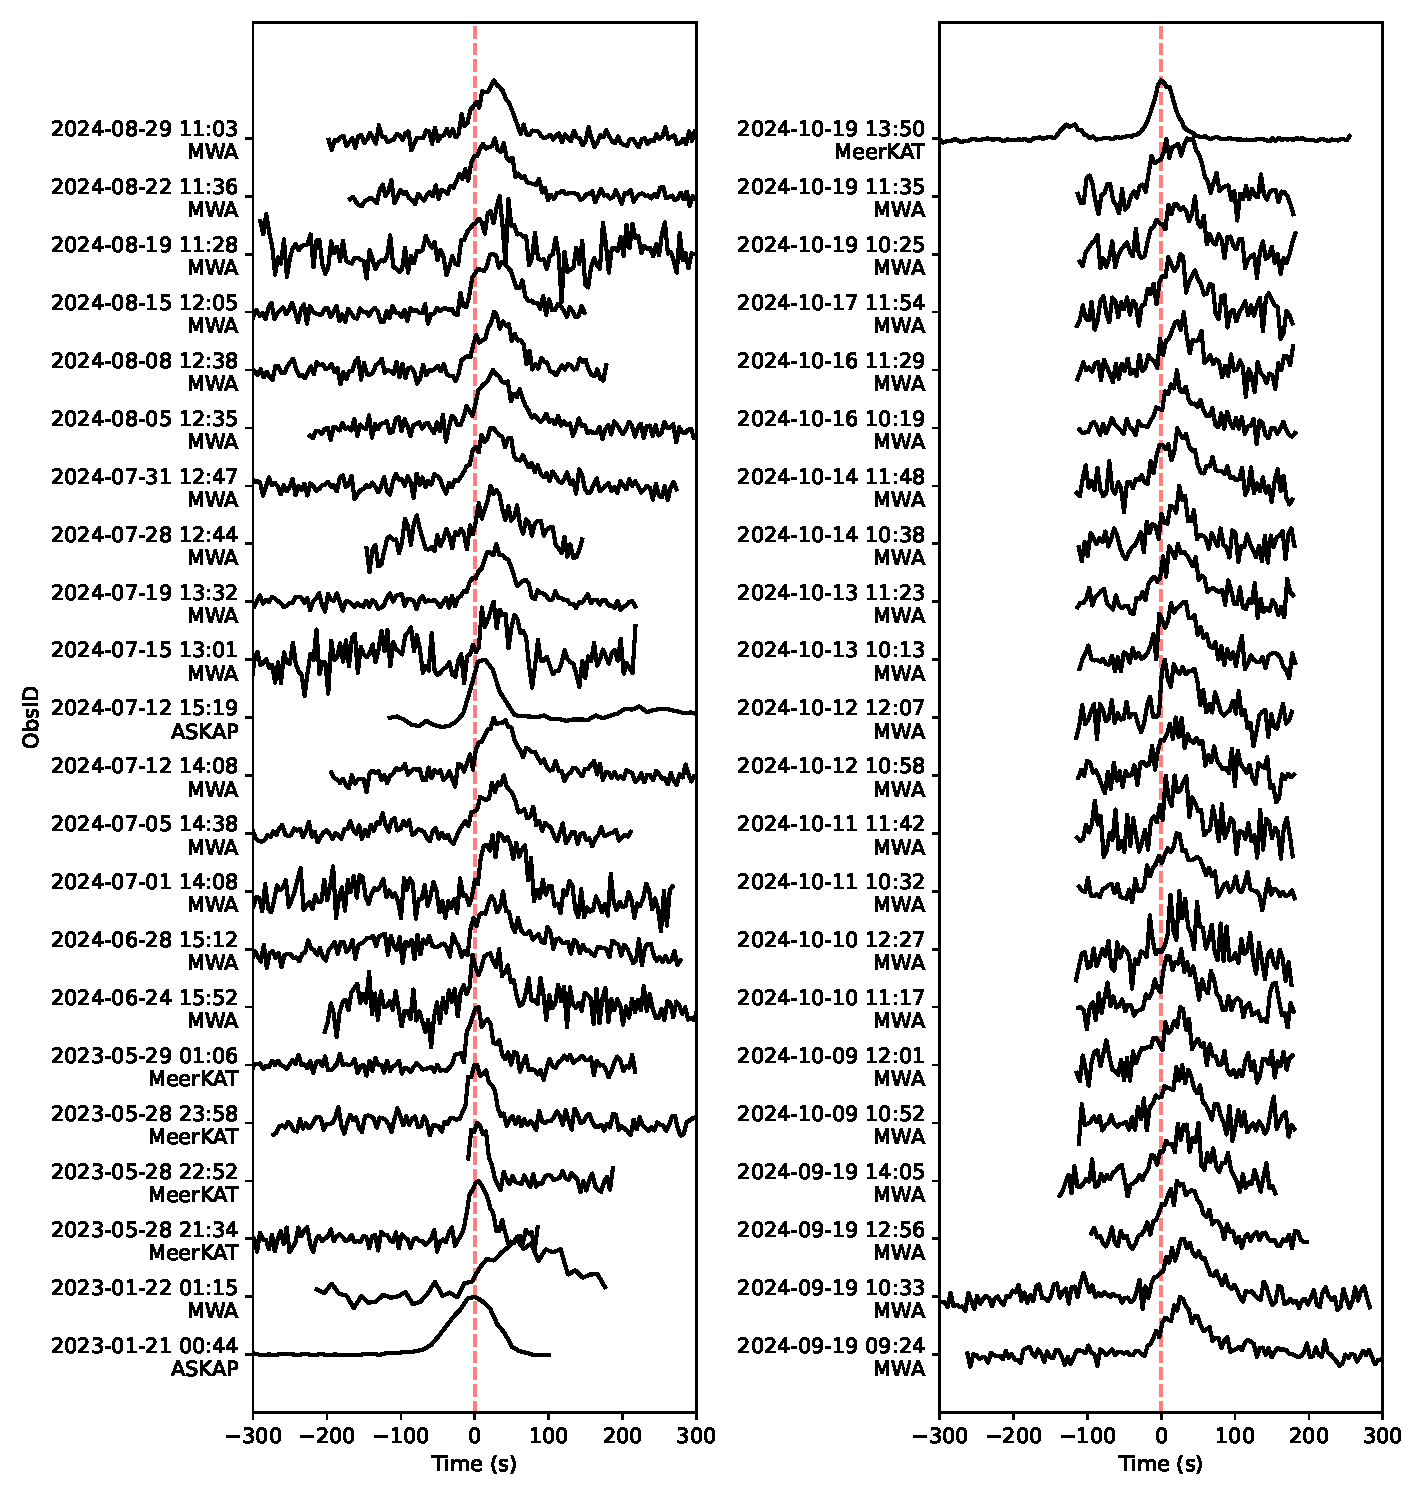
\includegraphics[width=0.95\linewidth]{pulsestack.pdf}
              \caption{Pulsestack of barycentred, dedispersed profiles from the ephemeris. The dashed red vertical line marks zero phase. Baselines have been fitted and subtracted from each lightcurve. The blue dashed lines show (normalised) fitted Gaussians without scattering (see main text for details).}
                  \label{fig:pulsestack}
\end{figure*}

For the MeerKAT pulse with two components, we fit only the brighter component.

\subsection{Timing solution} \label{sec:timing}

Because the large scattering time scale at low frequencies significantly distorts the pulse shapes, common methods for defining ToAs can potentially result in systematic errors of up to tens of seconds, as discussed in detail in Appendix \ref{app:scattering_dm}.
These systematic errors set up a degeneracy between DM and scattering time scales that is not easily disambiguated.

This is demonstrated in \Fig~\ref{fig:stacked_spectra}, which shows stacked MWA and MeerKAT spectra.
The cyan lines show the expected ToAs across the whole observed frequency range if one assumes only a DM measured at higher frequencies, where scattering is negligible.
The scattering predicted by Galactic electron density models, however, is sufficient to account for the apparent extra delay, as is evidenced by the relatively good agreement with the modelled unscattered pulses with the expected ToAs derived from the ephemeris, illustrated in the pulsestack shown in \Fig~\ref{fig:pulsestack}.

\begin{figure}{th}
      \centering
          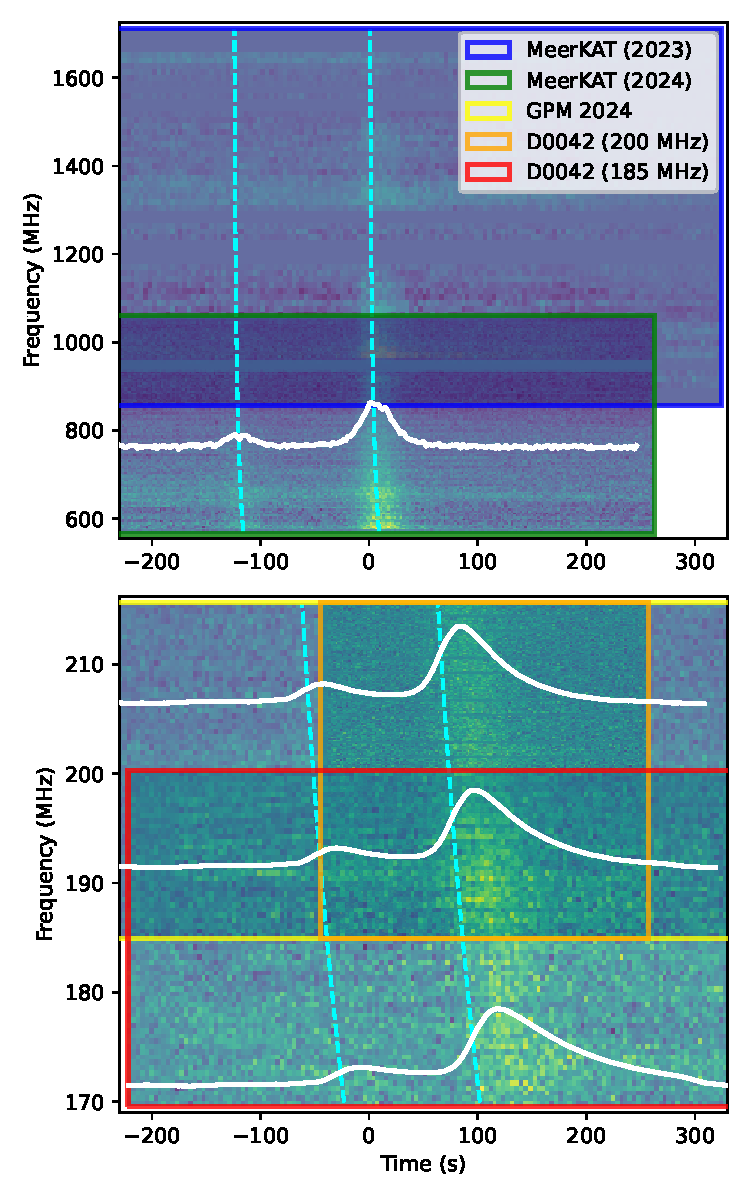
\includegraphics[width=0.95\linewidth]{stacked_spectra.pdf}
              \caption{Stacked (semi-transparent) dynamic spectra, where each rectangle indicates the observing campaign whose spectra were barycentred and folded according to the ephemeris. The spectra have not been dedispersed, but the cyan dashed lines indicate where the two components seen in the MeerKAT (2024) observation would appear due to dispersion. The white curve in the top panel is the dedispersed profile of the MeerKAT (2024) observation, and the white curves in the bottom panel are the same profile subjected to scattering with $\tau_{\rm sc} = \tau_{\rm sc,1\,GHz} (\nu/{\rm 1\,GHz})^{-4}$ at frequencies 175, 195, and 210 MHz, where $\tau_{\rm sc,1\,GHz} = 0.07\,$s.}
                  \label{fig:stacked_spectra}
\end{figure}

We therefore identified the times of arrival (ToAs) with the $\mu$ parameter in the fits given in Eq. \eqref{eqn:emg}, which represents the location of the assumed Gaussian pulse before scattering.
Because the scattering time scale could not be reliably measured for all individual pulses, we obtained ToAs by assuming a fixed scattering time of $\tau_{\rm sc,1 GHz} = 0.07\,$s.

%\begin{deluxetable*}{ccccc}
%  \tablecaption{Times of arrival and pulse properties\label{tbl:toas}}
%  \tablehead{
%    \colhead{Telescope} & \colhead{$\nu$} & \colhead{ToA} & \colhead{Fluence} & \colhead{$\sigma$} \\ 
%    & \colhead{(MHz)} & \colhead{(MJD)} & \colhead{($10^3$\,Jy\,s)} & \colhead{(s)}
%  } 
%  \startdata
%ASKAP & 888 & 59965.0429358(45) & 0.48(2) & 29.1(4) \\
%MWA & 170 & 59966.061584(40) & 31.7(7) & 40(7) \\
%ASKAP & 888 & 60040.913447(32) & 0.03(1) & 25(3) \\
%MeerKAT & 1284 & 60092.899548(10) & 0.003(3) & 13(1) \\
%MeerKAT & 1284 & 60092.947966(10) & 0.003(3) & 12(1) \\
%MeerKAT & 1284 & 60092.996466(11) & 0.005(3) & 16(1) \\
%MeerKAT & 1284 & 60093.044919(12) & 0.005(4) & 16(1) \\
%MWA & 200 & 60481.637466(65) & 3.0(2) & 24(8) \\
%MWA & 200 & 60485.658977(33) & 1.18(7) & 16(4) \\
%MWA & 200 & 60489.632266(20) & 1.65(6) & 14(2) \\
%MWA & 200 & 60492.588020(24) & 3.12(9) & 14(3) \\
%MWA & 200 & 60496.609639(18) & 2.87(8) & 17(2) \\
%MWA & 200 & 60503.587085(14) & 3.40(8) & 17(2) \\
%ASKAP & 1032 & 60503.634781(17) & 0.09(1) & 16.6(5) \\
%MWA & 200 & 60506.542809(33) & 1.35(6) & 9(4) \\
%MWA & 200 & 60510.564531(11) & 3.08(7) & 16(1) \\
%MWA & 200 & 60519.528812(29) & 3.1(1) & 14(4) \\
%MWA & 200 & 60522.533028(16) & 3.50(8) & 18(2) \\
%MWA & 200 & 60527.524033(14) & 2.89(7) & 16(2) \\
%MWA & 200 & 60530.528339(16) & 2.90(8) & 17(2) \\
%MWA & 200 & 60537.506042(13) & 3.91(9) & 17(2) \\
%MWA & 200 & 60541.479448(47) & 1.48(9) & 14(5) \\
%MWA & 200 & 60544.483761(15) & 3.91(9) & 20(2) \\
%MWA & 200 & 60551.461625(16) & 3.35(8) & 16(2) \\
%MWA & 185 & 60572.395455(15) & 2.86(7) & 15(2) \\
%MWA & 185 & 60572.443943(21) & 3.01(8) & 16(2) \\
%MWA & 185 & 60572.540824(18) & 2.57(8) & 16(2) \\
%MWA & 185 & 60572.589281(31) & 4.3(2) & 21(4) \\
%MWA & 200 & 60592.456765(27) & 1.63(8) & 19(3) \\
%MWA & 200 & 60592.505159(33) & 1.67(9) & 19(4) \\
%MWA & 200 & 60593.474369(26) & 1.08(6) & 15(3) \\
%MWA & 200 & 60593.522901(46) & 1.3(1) & 19(5) \\
%MWA & 200 & 60594.443484(20) & 1.94(8) & 18(2) \\
%MWA & 200 & 60594.491990(33) & 0.55(5) & 12(4) \\
%MWA & 200 & 60595.461118(29) & 1.53(8) & 19(3) \\
%MWA & 200 & 60595.509617(25) & 0.89(5) & 13(3) \\
%MWA & 200 & 60596.430282(20) & 1.55(7) & 16(2) \\
%MWA & 200 & 60596.478721(23) & 1.65(7) & 17(3) \\
%MWA & 200 & 60597.447846(41) & 0.86(7) & 16(5) \\
%MWA & 200 & 60597.496319(30) & 1.82(9) & 19(3) \\
%MWA & 200 & 60599.434635(17) & 1.28(5) & 13(2) \\
%MWA & 200 & 60599.483121(24) & 1.00(5) & 13(3) \\
%MWA & 200 & 60600.500655(31) & 1.24(7) & 16(4) \\
%MWA & 200 & 60602.438964(32) & 1.9(1) & 21(4) \\
%MWA & 200 & 60602.487394(27) & 1.98(9) & 20(3) \\
%MeerKAT & 813 & 60602.5835731(40) & 0.061(7) & 14.9(4)
  %\enddata
%\end{deluxetable*}

These ToAs were then barycentred and fit for both period and DM, resulting in the values given in \Tab~\ref{tbl:ephemeris}.
The residuals are plotted in \ref{fig:pulse_details}, along with the fitted pulse widths and fluences.
We also tried fitting a timing model that included a spin-down parameter, and found that it was consistent with zero spin-down to within $1\sigma$, and so is not included in the ephemeris.

\begin{table}
  \centering
  \caption{Timing ephemeris for \src{}}
  \label{tbl:ephemeris}
  \begin{tabular}{lc}
    \hline
    Parameter & Value \\
    \hline
    Period (s) & $4186.3283 \pm 0.0003$ \\
    PEPOCH (MJD) & $59965.03790 \pm 0.00003$ \\
    DM (pc/cm$^{-3}$) & $764 \pm 25$ \\
    $\tau_{\rm sc,1 GHz}$ (s) & ${\sim}0.07$ \\
    \hline
  \end{tabular}
\end{table}

\begin{figure*}{th}
  \centering
  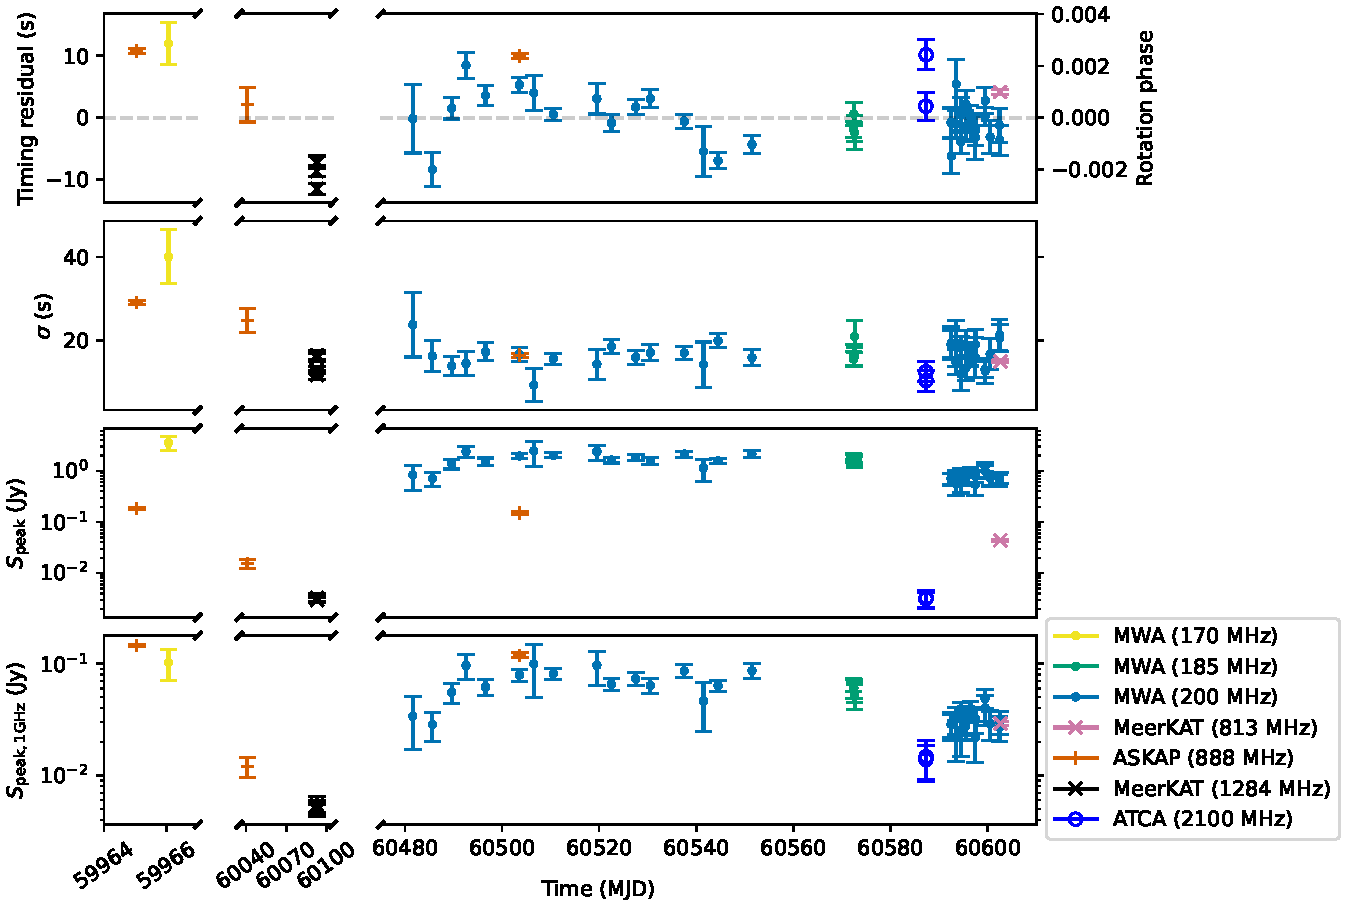
\includegraphics[width=0.98\linewidth]{pulse_details.pdf}
  \caption{Timing residuals (top panel) and other pulse properties derived from the fits of Eq. \eqref{eqn:emg} to the individual light curves (lower two panels). \dots}
  \label{fig:pulse_details}
\end{figure*}

The measured DM of $764 \pm 25\,{\rm pc}\,{\rm cm}^{-3}$ is slightly higher than, but still consistent with, the in-band measurement of $710^{+200}_{-180}\,{\rm pc}\,{\rm cm}^{-3}$ given in \citetalias{2024MNRAS.535..909D}.
Because we have not attempted to simultaneously fit for both DM and scattering timescale, there will remain some small systematic error on this reported DM measurement.
Breaking the degeneracy is possible in principle with a much higher S/N average profile than what is achievable with the current data set.

For planning observations of \src{} at low ($\lesssim 300 MHz$), care should be taken to incorporate scattering into the predicted ToAs.
The $N$th pulse since PEPOCH is predicted to arrive at the Solar System barycentre at
\begin{equation}
    {\rm MJD} = {\rm PEPOCH} + NP + \Delta t_{\rm DM}(\nu) + \Delta t_{\rm sc}(\nu),
\end{equation}
where PEPOCH and the period, $P$, are given in \Tab~\ref{tbl:ephemeris},
\begin{equation}
    \Delta t_{\rm DM}(\nu) = 4148\,{\rm s} \, \left(\frac{\rm DM}{{\rm pc\,cm}^{-3}}\right) \left(\frac{\nu}{\rm MHz}\right)^{-2}
\end{equation}
is the usual dispersion attributed to the interstellar medium, and
\begin{equation}
    \Delta t_{\rm sc}(\nu) = -\sqrt{2}\sigma\erfcx^{-1}\left(\frac{\tau(\nu)}{\sigma}\sqrt{\frac{2}{\pi}}\right) + \frac{\sigma^2}{\tau(\nu)}
    \label{eqn:scattering_delay}
\end{equation}
is the amount that the \emph{peak} of the observed pulse is delayed by scattering.
When calculating this quantity, we recommend using $\sigma = 15\,$s, a typical value for low-frequency pulses (see \Fig~\ref{fig:pulse_details}).
At frequencies above $300\,$MHz, $\tau(\nu) \ll \sigma$, and the delay due to scattering, which asymptotically behaves like $\Delta t_{\rm sc}(\nu) \sim \tau$, can be safely neglected.
At frequencies below $150\,$MHz, the asymptotic behaviour
\begin{equation}
    \Delta t_{\rm sc}(\nu) \sim \sigma \sqrt{\ln \left(\frac{\tau^2}{2\pi \sigma^2}\right)} + \frac{\sigma^2}{\tau}
\end{equation}
is accurate to within a few seconds.
At intermediate frequencies ($150\,{\rm MHz} \lesssim \nu \lesssim 300\,{\rm MHz}$), Eq. \eqref{eqn:scattering_delay} should be used directly.

%Following the positive identification of several pulses in the GPM data set, we performed a grid search of periods that would result in an integer number of pulses between two widely spaced pulses.
%A candidate period of $P = 4186.4 \pm 0.1$ was found for which all detections fell within a narrow window of ${\sim}0.05$ of phase.
% We further refined this by attempting to phase connect to Dougal's original pulse, and got $4186.33 \pm 0.02$ s, but this needn't be part of the story, since even the above was enough to motivate the MWA campaign that followed.
%This motivated the follow-up MWA observations (under project code D0042) in which two consecutive pulses ${\sim}4190$ seconds apart were detected without any discernible emission between them, ruling out periods $P/n$, for $n \ge 2$.
%The lever arm afforded by both the GPM and D0042 detections proved sufficient to phase-connect to the original pulse published by \citetalias{2024MNRAS.535..909D}, yielding a refined period of $P = 4186.33 \pm 0.02$~s.

%We then measured times of arrival (ToAs) of individual pulses.
%The ASKAP and MWA pulses were morphologically similar and well fit by a simple Gaussian.

\subsection{Polarization} \label{sec:polarization}

No significant polarised emission was detected in the MWA pulses, as well as the 2023 MeerKAT pulses.
The apparent lack of polarisation in the MeerKAT data set is likely due to low S/N coupled with the source not being not being centred in the beam.
Much more careful analysis would be needed to obtain reliable limits on the polarised components of those pulses.

The apparent lack of linear polarisation in the MWA pulses, however, is expected due to the high RM of ${\sim}961\,{\rm rad}/{\rm m}^2$ \citepalias[as reported in][]{2024MNRAS.535..909D}, causing the pulses to be depolarised within individual channels.
We also report that no significantly circularly polarised emission was seen at MWA frequencies.

The three sufficiently bright pulses for which we report significant polarisation are (1) the original 2023 ASKAP pulse \citepalias{2024MNRAS.535..909D}, (2) the 2024 ASKAP pulse, and (3) the 2024 MeerKAT pulse.
We applied the parallactic angle correction to the MeerKAT data, as this had not already been applied during upstream processing.

The high S/N of each time bin allowed us to test whether the rotation measure (RM) was consistent across each pulse.
We therefore performed a joint fit of the Stokes Q and U spectra of each time bin to
\begin{equation}
    Q(\nu) = {\rm Re}(\mathcal{L}(\nu)),
    \quad
    U(\nu) = {\rm Im}(\mathcal{L}(\nu)),
    \label{eqn:RM}
\end{equation}
where
\begin{equation}
    \mathcal{L}(\nu)
        = L_{\rm 1\,GHz}\left(\frac{\nu}{\rm 1\,GHz}\right)^{\alpha_L} e^{2i({\rm RM}\,\lambda^2 + \psi_0)},
\end{equation}
$L_{\rm 1\,GHz}$ is the flux density of the linearly polarised component at 1\,GHz, $\alpha_L$ is its spectral index, RM is the rotation measure, $\lambda = c/\nu$ is the wavelength, and $\psi_0$ is the intrinsic polarisation angle.
The RMs and spectral indices of these fits are shown in the top two rows of panels of \Fig~\ref{fig:RM}.

\begin{figure*}{th}
    \centering
    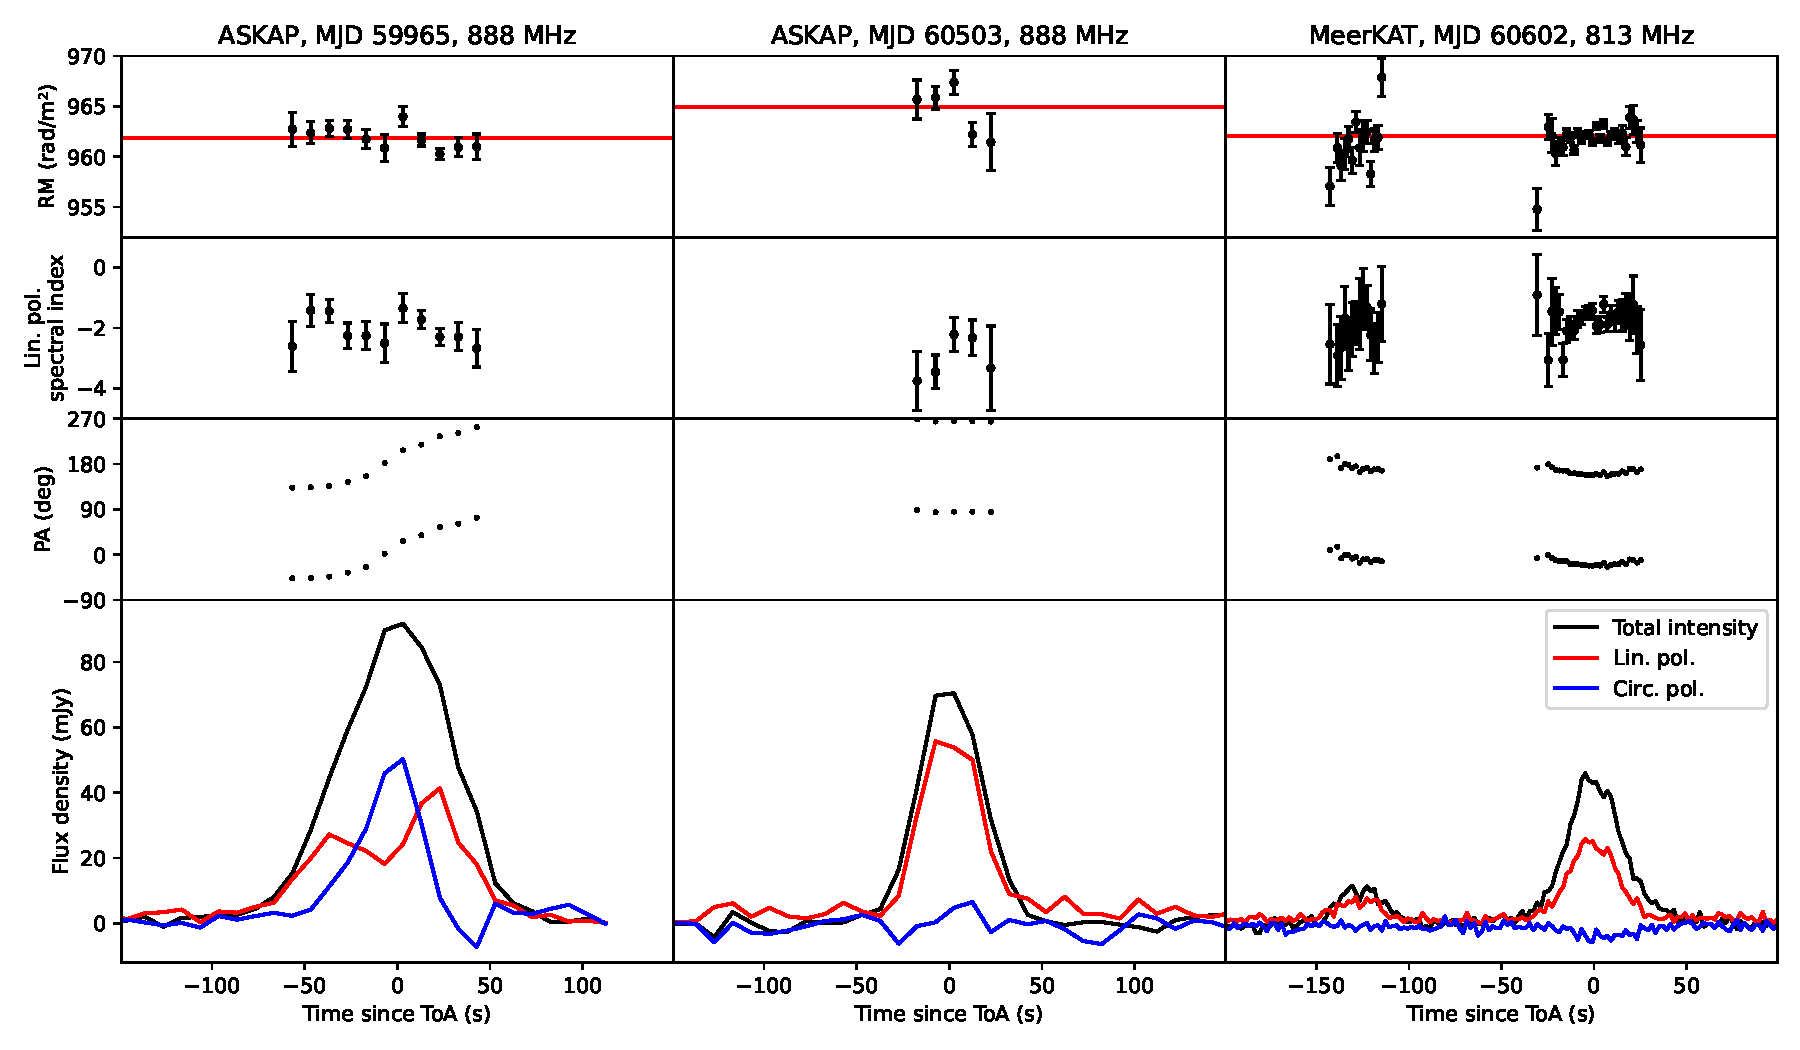
\includegraphics[width=0.98\linewidth]{RM.pdf}
    \caption{Polarisation of the 2023 and 2024 ASKAP pulses (left and middle) and the 2024 MeerKAT pulse (right). The top two rows show the RM and $\alpha_{\rm lin}$ parameters fitted to Eq. \eqref{eqn:RM} for each time bin independently. Only bins for which the uncertainty on $\alpha_{\rm lin}$ is less than $1.4$ are shown, a threshold which was found to cleanly eliminate off-pulse bins. The weighted average RMs for each pulse are indicated by the horizontal red lines. The PAs and lightcurves shown in the bottom two rows of panels were produced using only the average RM for the respective pulse.}
    \label{fig:RM}
\end{figure*}

We found that the RM derived for the MeerKAT pulse had the opposite sign, but similar magnitude, to the ASKAP pulses, which is most likely due to a different sign convention being used within the two telescopes' pre-processing software.
The agreement presented in \Fig~\ref{fig:RM} was achieved by first negating Stokes Q in the MeerKAT data.
Any reflection in the Q-U plane (e.g. ${\rm Q} \leftrightarrow -{\rm Q}$, ${\rm U} \leftrightarrow -{\rm U}$, or ${\rm Q} \leftrightarrow {\rm U}$) will achieve a similar correction to the sign of the RM, but different choices will introduce different offsets to the PA.
Because of this, the MeerKAT PA values should not be directly compared with the ASKAP values.
The most likely scenario, however, is that the MeerKAT values include an arbitrary offset of $n \times 45^\circ$, for some integer $n$.

In all cases, the magnitude of the fitted RM was within a few rad/m$^2$ of the value originally derived for the 2023 ASKAP pulse in \citetalias{2024MNRAS.535..909D}.
The RM appears to decrease slightly over the course of the 2023 ASKAP pulse, and \emph{increase} slightly over the course of the two 2024 MeerKAT components; however, all values are consistent with a constant RM across all three pulses.
The per-pulse weighted averaged values (with weighting proportional to the Stokes I profile) are $962 \pm 1$\,${\rm rad}/{\rm m}^2$ (2023 ASKAP), $965 \pm 2$ (2024 ASKAP) and $962 \pm 2$\,${\rm rad}/{\rm m}^2$ (2024 MeerKAT).
The spectral index of the linear component, $\alpha_L$, is similarly consistent, with averages value of $-2.1 \pm 0.4$ (2023 ASKAP), $-3.0 \pm 0.6$ (2024 ASKAP) and $-1.9 \pm 0.5$ (2024 MeerKAT).

Each pulse was de-Faraday rotated with the weighted average RM given above, to derive the linear polarisation profile and the PA evolution across the pulses.
For the 2023 ASKAP pulse, we recover the `S'-shaped PA curve discussed at length in \citetalias{2024MNRAS.535..909D} in the context of the RVM.
Contrastingly, the PA curve of the 2024 ASKAP pulse is flat (across five 10-second bins), and that of the 2024 MeerKAT pulse is curved, but not in an RVM-like way.

\section{Discussion} \label{sec:discussion}

After accounting for dispersion and scattering effects, the timing analysis of \src{} confirms its status as an LPT, as originally conjectured in \citetalias{2024MNRAS.535..909D}.
It has the fifth largest period (${\sim}1.16\,$hours) of known published LPTs, after ASKAP J1839$-$0756 \citep[$6.45\,$hours;][]{Lee2025}, GLEAM-X J0704$-$37 \citep[$2.92\,$hours;][]{2024ApJ...976L..21H,2025A&A...695L...8R}, ILT J1101+5521 \citep[$2.09\,$hours;][]{deRuiter2025}, and GCRT J1745$-$3009 \citep[$1.28\,$hours;][]{2005Natur.434...50H}.

With the timing solution in hand, we can explore the efficacy of the original follow-up campaign described in \citetalias{2024MNRAS.535..909D}.
Assuming \src{} remained at a similar brightness (see \Fig~\ref{fig:pulse_details}), it should have been detected in two ASKAP observations (2023-04-06 and 2023-10-18) and a few dozen times throughout the MWA's 2022 GPM run (2022-06-02 to 2022-09-08).
There are also three observations in the earliest part of the 2024 GPM run (one on 2024-06-02 and two on 2024-06-10) in which no pulse was observed.
However, pulses were detected just ten days later on 2024-06-20 (the first of the MWA 200\,MHz points in \Fig~\ref{fig:pulse_details}), and at each epoch thereafter whenever the MWA was observing in \src{}'s direction when a pulse was due to arrive.

We conclude, therefore, that \src{} is intermittent with active periods lasting on the order of months, and that the most recent activity period fortuitously started shortly after the start of the 2024 GPM observation run.
The entire set of observations presented in this work, spanning from 2023 to 2024, may represent two or three different activity windows.
This is reminiscent of the behaviour of GLEAM-X J162759.5$-$523504.3, which was ``on'' in January 2020, ``off'' in Feburary, and ``on'' again in March \citep{2022Natur.601..526H}.
The periodic (or quasi-periodic) reappearance of \src{} suggests the possibility that other known intermittent LPTs (like GLEAM-X J162759.5$-$523504.3 and GCRT J1745$-$3009) may eventually do likewise.

As noted in \citetalias{2024MNRAS.535..909D}, optical follow-up of \src{} is hampered by its proximity to the Galactic plane ($b = -0.12^\circ$).
Inferring this nature of the system (white dwarf vs neutron star, isolated vs binary) from the radio pulses alone is challenging, unless either the population of LPTs is better understood as a whole, or if some other property of the radio signal (e.g. intermittency, polarisation) can be linked to the system properties.

\src{}'s period and duty cycle are not dissimilar to ILT J1101+5521 and GLEAM-X J0704$-$37, which are confirmed polars (\Fig~\ref{fig:lpt_comparison}), suggesting the possibility that \src{}, too, is a WD-MD polar system.
However, its period of ${\sim}1.16\,$hours would make it shorter than the minimum known orbital period of $1.3\,$hours for confirmed polars \citep{schwope2025polarcatcatalogpolarslowaccretion}.
This makes it an interesting testbed for the suggestion advanced by \citet{2025A&A...695L...8R} that ``short LPTs'' ($P \lesssim 78\,$mins) and ``long LPTs'' ($P \gtrsim 78\,$mins) represent different classes of systems (AM CVns and CVs, respectively).
\begin{figure*}{th}
    \centering
    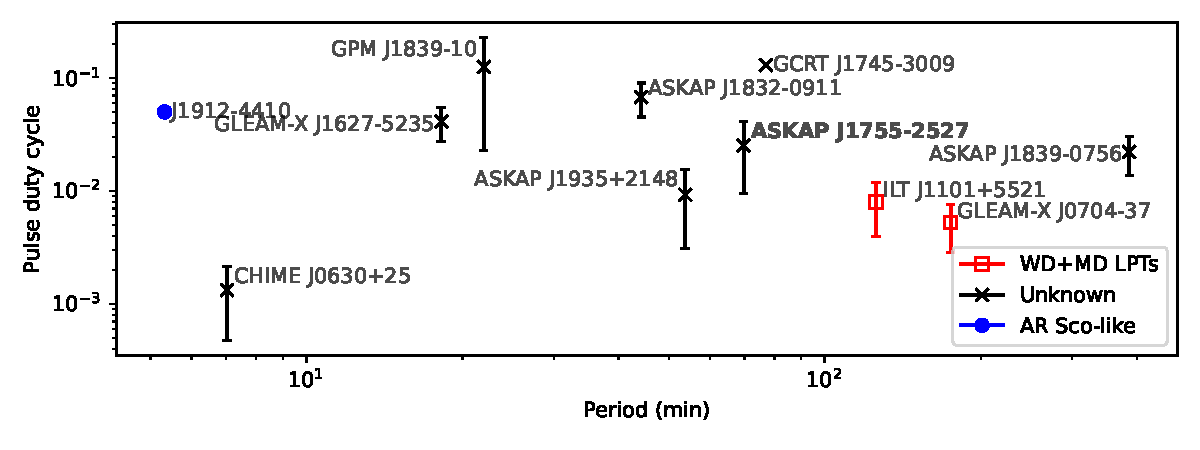
\includegraphics[width=0.98\linewidth]{lpt_comparison.pdf}
    \caption{Duty cycle vs radio pulse period for various classes of radio emitters \citep{deRuiter2025,2022Natur.601..526H,2023Natur.619..487H,2024NatAs...8.1159C,2005Natur.434...50H,deRuiter2025,Lee2025}. The duty cycles are derived from the reported pulse widths for LPTs, which are compared to the range of the fitted, unscattered pulse widths of \src{} at 10\% of the peak. AR\,Sco \citep{2016Natur.537..374M,2018A&A...611A..66S} and other sources without well-defined periods or duty cycles \citep[e.g.][and references therein]{2021ApJ...920...45W} are not included on this plot.}
    \label{fig:lpt_comparison}
\end{figure*}

%\begin{deluxetable*}{lcl}
%  \tablecaption{Known and candidate LPTs, arranged in ascending order of period\label{tbl:lpts}}
%  \tablehead{
%    \colhead{LPT} & \colhead{Period} & \colhead{References} \\ 
%     & \colhead{(min)} & 
%   } 
%   \startdata
%   %AR Scorpii (J162147.28-225310.3) & 1.97 &  \\
%   %ASKAP J175154.89-255135.3 & ${\sim}$3.6 &  \\
%   %J1912-4410 & 5.3 &  \\
%   CHIME J0630+25             & 7.02 & \citet{2024arXiv240707480D} \\
%   GLEAM-X J162759.5-523504.3 & 18.2 & \citet{2022Natur.601..526H} \\
%   GPM J1839-10               & 22.0 & \citet{2023Natur.619..487H} \\
%   ASKAP J1832-0911           & 44.3 & \todo{Wang} \\
%   ASKAP J193505.1+214841.0   & 53.8 & \citet{2024NatAs...8.1159C} \\
%   ASKAP J175534.9-252749.1   & 69.8 & \citetalias{2024MNRAS.535..909D} \\
%   GCRT J1745-3009            & 77.0 & \citet{2005Natur.434...50H} \\
%   ILT J1101+5521             & 126  & \citet{2024arXiv240811536D} \\
%   GLEAM-X J0704-37           & 175  & \citet{2024arXiv240815757H} \\
%   ASKAP J1839-0756           & 387  & \citet{Lee2025} \\
%   \enddata
%\end{deluxetable*}


Although there is as yet no clear consensus on whether LPTs represent one class or multiple classes of system \citep[e.g.][]{2024ApJ...961..214R}, the recent confirmation of J1912$-$4410 as a pre-evolved white dwarf pulsar \citep{2023NatAs...7..931P} and ILT\,J1101+5521 and GLEAM-X\,J0704$-$37 as polars \citep{deRuiter2025,2025A&A...695L...8R} raise the intriguing possibility that other LPTs may also be radio-emitting white dwarf pulsars at various stages of evolution \citep{2021NatAs...5..648S}.

In this view, the intermittency of these systems have several possible explanations.
The limited orbital phase range in which J1912$-$4410's radio pulses were observed suggests that the geometric configuration is important in the observability of radio pulsations; ``missing'' pulses may simply occur at unfavourable orbital phases.
This is readily testable with long-term monitoring---this kind of intermittency will have the same periodicity as the orbit itself.

Interestingly, systems with spin-orbital (or beat-orbital) resonances of, e.g., 2:1 or 3:1, coupled with the idea of a limited observable orbital phase window for the radio pulses, would be indistinguishable from systems in 1:1 resonances.
We therefore advance the possibility that the coincidence of the observed radio periodicities of ILT\,J1101+5521 and GLEAM-X\,J0704$-$37 with their spectroscopically confirmed orbital periods does not necessarily imply that they are 1:1 polars.

Similarly, systems in which the spin-orbit (or beat-orbit) ratios are \emph{close to} small-integer ratios, or, equivalently, systems in which precession of the WD is significant, will exhibit an extra beating effect in which an orbitally-induced intermittency is aliased to a much lower frequency.
The month-long time scale of the intermittency of \src{}, and possibly even GLEAM-X\,J1627$-$5235, may be of this kind; much longer-term monitoring is needed to confirm or refute this.

Another possibility is that radio emission is only observed when the MD produces dense enough particle outflows, in the form of winds, to activate the emission mechanism in the vicinity of the WD.
Such outflows can last for months [CITATION??], and would not be strictly periodic.
If intermittency is of this sort, then the observed activity windows will be similarly aperiodic, or quasiperiodic.
Again, long-term monitoring can help distinguish between these scenarios.



% SM: MEMO TO SELF: Add mention of early 2023 pulses being wider (and brighter) than all others. Note also the spectral index roughly staying the same, and state a number of roughly what that is by comparing low- and high- frequency flux densities ratios. All this can probably go in Analysis/Results above rather than discussion.



%%%%% Discussion of MeerKAT precursor %%%%%
%The precursor burst seen with MeerKAT is apparently unique, and is not visible at other telescopes and frequencies, even after averaging them together to make a single profile.
%The only burst of comparable S/N, and at a similar frequency, in which the dimmer precursor component might be expected to be visible is the original 2023-01-21 ASKAP burst \citepalias{2024MNRAS.535..909D}, where again it is absent.
%...

%%%%% Discussion of brighter pulses in 2023 %%%%%
%The two pulses observed in January 2023 (the original ASKAP pulse and the MWA (IPS) pulse observed the following day) are significantly wider than all other pulses, suggesting that a morphological change occurred between ...

%%%%% Other things to possibly discuss:
% - Qu & Zhang #2: https://ui.adsabs.harvard.edu/abs/2025ApJ...981...34Q/abstract
% - Gaia22ayj: https://ui.adsabs.harvard.edu/abs/2025PASP..137b4202R/abstract
% - Trying to find a number for the radio duty cycle of AR Sco
%   - This one's about the pair-wise alternation of (optical?) pulse brightnesses, and an interpretation involving precession: https://ui.adsabs.harvard.edu/abs/2023ApJ...958L..22G/abstract
%   - Fancy AR Sco modelling. Magnetic mirror models are mentioned in the abstract? https://ui.adsabs.harvard.edu/abs/2025arXiv250508567D/abstract
%   - Ok, I think this is as good as it gets: Stanway 2018 (reference already imported into biblio.bib.
% - https://ui.adsabs.harvard.edu/abs/2022Ap%26SS.367..108K/abstract
% - Suggestion that J1627 is a WD pulsar: https://ui.adsabs.harvard.edu/abs/2022Ap%26SS.367..108K/abstract

%\begin{enumerate}
%        \item Why does the source appear to not be active all the time at higher frequencies?
%              \item As per convo with John (see MWA Users Slack, 2025-01-24), point out that (lack of detection of source in) MWA IPS is not very constraining in terms of scattering disk / timescale / screen.
%\end{enumerate}


\section{Summary} \label{sec:summary}

We have shown that \src{} is in fact an LPT, as conjectured in \citetalias{2024MNRAS.535..909D}).
Its period of ${\sim}1.16\,$hours is slightly shorter than the minimum known orbital\dots

\section*{Acknowledgements}

N.H.-W. is the recipient of an Australian Research Council Future Fellowship (project number FT190100231).
 
 This scientific work uses data obtained from Inyarrimanha Ilgari Bundara, the CSIRO Murchison Radio-astronomy Observatory. Support for the operation of the MWA is provided by the Australian Government (NCRIS), under a contract to Curtin University administered by Astronomy Australia Limited. ASVO has received funding from the Australian Commonwealth Government through the National eResearch Collaboration Tools and Resources (NeCTAR) Project, the Australian National Data Service (ANDS), and the National Collaborative Research Infrastructure Strategy.
% Skipped because it is acknowledged below.
% We acknowledge the Pawsey Supercomputing Centre which is supported by the Western Australian and Australian Governments.
% ASKAP -- I have fixed this to use the correct name for the observatory
The Australian SKA Pathfinder is part of the Australia Telescope National Facility which is managed by CSIRO. Operation of ASKAP is funded by the Australian Government with support from the National Collaborative Research Infrastructure Strategy. ASKAP and the MWA use the resources of the Pawsey Supercomputing Centre. Establishment of ASKAP, Inyarrimanha Ilgari Bundara, and the Pawsey Supercomputing Centre are initiatives of the Australian Government, with support from the Government of Western Australia and the Science and Industry Endowment Fund. We acknowledge the Wajarri Yamaji People as the Traditional Owners and Native Title Holders of the observatory site.

% MeerKAT
The MeerKAT telescope is operated by the South African Radio Astronomy Observatory, which is a facility of the National Research Foundation, an agency of the Department of Science and Innovation.
  % PTUSE (https://skaafrica.atlassian.net/wiki/spaces/ESDKB/pages/1591672833/User+Supplied+Equipment+USE#PTUSE)
  Observations made use of the Pulsar Timing User Supplied Equipment (PTUSE) servers at MeerKAT which were funded by the MeerTime Collaboration members ASTRON, AUT, CSIRO, ICRAR-Curtin, MPIfR, INAF, NRAO, Swinburne University of Technology, the University of Oxford, UBC and the University of Manchester.  The system design and integration was led by Swinburne University of Technology and Auckland University of Technology in collaboration with SARAO and supported by the ARC Centre of Excellence for Gravitational Wave Discovery (OzGrav) under grant CE170100004.

%%%%%%%%%%%%%%%%%%%%%%%%%%%%%%%%%%%%%%%%%%%%%%%%%%
\section*{Data Availability}

\dots
 
%The inclusion of a Data Availability Statement is a requirement for articles published in MNRAS. Data Availability Statements provide a standardised format for readers to understand the availability of data underlying the research results described in the article. The statement may refer to original data generated in the course of the study or to third-party data analysed in the article. The statement should describe and provide means of access, where possible, by linking to the data or providing the required accession numbers for the relevant databases or DOIs.



%%%%%%%%%%%%%%%%%%%% REFERENCES %%%%%%%%%%%%%%%%%%

% The best way to enter references is to use BibTeX:

\bibliographystyle{mnras}
\bibliography{biblio} % if your bibtex file is called example.bib


% Alternatively you could enter them by hand, like this:
% This method is tedious and prone to error if you have lots of references
%\begin{thebibliography}{99}
%\bibitem[\protect\citeauthoryear{Author}{2012}]{Author2012}
%Author A.~N., 2013, Journal of Improbable Astronomy, 1, 1
%\bibitem[\protect\citeauthoryear{Others}{2013}]{Others2013}
%Others S., 2012, Journal of Interesting Stuff, 17, 198
%\end{thebibliography}

%%%%%%%%%%%%%%%%%%%%%%%%%%%%%%%%%%%%%%%%%%%%%%%%%%

%%%%%%%%%%%%%%%%% APPENDICES %%%%%%%%%%%%%%%%%%%%%

\appendix

\section{The effect of scattering on timing}
\label{app:scattering_dm}

It can be shown that pulses scatter-broadened by a thin screen will appear to the observer as the original pulse convolved with a one-sided exponential kernel with an associated timescale $\tau$ [CITATION].
For intrinsically Gaussian pulses of scale $\sigma$, the result of this convolution is well described by the \textit{exponentially modified Gaussian} (EMG), as given in Eq. \eqref{eqn:emg}.

In the regime $\tau \ll \sigma$, the effect of scattering is negligible and the scattered pulse resembles the original pulse.
ToAs can be obtained in the usual way, i.e., using a matched filter ``template'' constructed from the average pulse profile.

On the other hand, in the regime $\tau \gg \sigma$, the leading edge of the EMG rises sharply (resembling the error function, $\erf$) and the trailing edge resembles the exponential kernel itself.
For this reason, pulse ToAs are typically mapped to the rising edge of highly scattered pulses, which closely approximates the centre of the original unscattered pulse.

In this appendix, we discuss the effect of scattering on measuring a DM from pulse observations if scattering is not taken into account.
As will be shown, the effect is most dramatic when $\tau \approx \sigma$, and in the case of wide, highly scattered pulses from LPTs like \src{}, can lead to a discrepant DM measurement of several hundreds of pm\,cm$^{-3}$.

We consider four methods for defining ToAs:
\begin{subequations}
(1) the position where the leading edge reaches half-maximum (LEHM),
\begin{equation}
    \emg(\ToA{LEHM}) = \frac{1}{2} A\exp\left(-\frac{1}{2}\left(\frac{\mu - t_m}{\sigma}\right)^2\right),
\end{equation}
where
\begin{equation*}
    t_m = \mu - \sqrt{2}\sigma\erfcx^{-1}\left(\frac{\tau}{\sigma}\sqrt{\frac{2}{\pi}}\right) + \frac{\sigma^2}{\tau^2}
\end{equation*}
is the mode of the EMG,
(2) the inflection point on the leading edge (IPLE),
\begin{equation}
    \left.\dd{\emg(t)}{t}\right|_{t = \ToA{IPLE}} = 0,
\end{equation}
(3) the position of the peak of the pulse (PEAK),
\begin{equation}
    \ToA{PEAK} = t_m,
\end{equation}
and (4) the maximum of the convolution of the pulse with a Gaussian profile with scale $\sigma$ (TMPL)
\begin{equation}
    \left.\deriv{}{t}\left(\emg(t) \ast \exp\left[ -\frac{1}{2} \left(\frac{t - \mu}{\sigma}\right)^2 \right]\right)\right|_{t = \ToA{TMPL}} = 0.
\end{equation}
The last definition is akin to template matching with a high-frequency (negligibly scattered) pulse profile.
\end{subequations}

None of the methods is entirely accurate in the presence of scattering.
We define the errors of the ToAs to be the difference between the measured ToA and the mean of the unscattered pulse,
\begin{equation}
    \Delta \ToA{} \equiv \ToA{} - \mu.
\end{equation}
For LEHM and IPLE, the ToA is measured to be earlier than $\mu$ ($\Delta{\rm ToA} < 0$); for PEAK and TMPL, later ($\Delta{\rm ToA} > 0$).
$\ToA{LEHM}$ and $\ToA{IPLE}$ will perform much better than $\ToA{PEAK}$ and $\ToA{TMPL}$ highly scattered pulses ($\tau \gg \sigma$), whereas the converse is true when scattering is minimal ($\tau \ll \sigma$).
All methods, however, perform relatively poorly in the intermediate regime when $\tau \approx \sigma$.

\begin{figure*}{th}
    \centering
    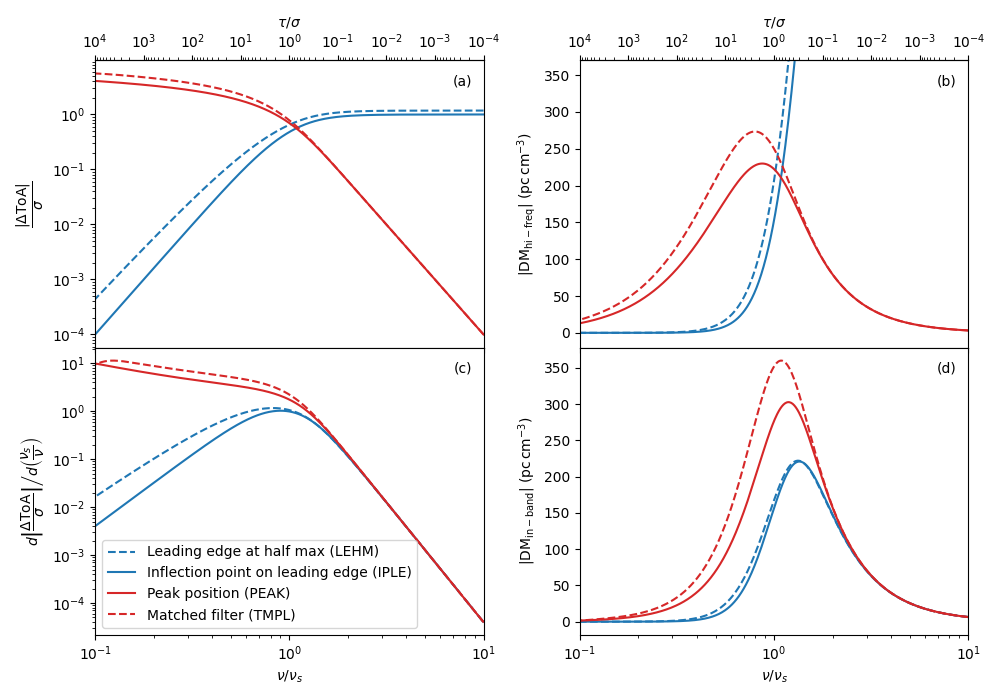
\includegraphics[width=0.98\linewidth]{scattering_DM.png}
    \caption{Analysis of DM measurement errors if scattering is not properly taken into account. Panel (a) shows the errors measured for each defined type of ToA, normalised to the scale of the original pulse, $\sigma$. In panel (b), the predicted error in DM is shown if the ToA error (compared to a high-frequency ToA measurement) is erroneously attributed to dispersion. Panel (c) shows the rate of change of the ToA error with frequency, and panel (d) shows the error in DM measured if this rate of change (the ``slope'' of the pulse across the observed dynamic spectrum) is erroneously attributed to dispersion. In panels (c) and (d), the derived DM errors assume a pulse scale of $\sigma = 25\,$s and $\nu_s = 230\,$MHz, as estimated for \src{}. In all panels, the blue curves indicate \emph{negative} ToA errors (i.e. the measured ToAs are earlier than the pulse's unscattered mean, $\mu$), and the red curves indicate positive quantities.}
    \label{fig:scattering_DM}
\end{figure*}

We computed numerically \citep[using SciPy's \texttt{root} function;][]{2020NatMe..17..261V} the errors for the four ToA types defined above, in the regime around $\tau \approx \sigma$.
These are shown in the panel (a) of \Fig~\ref{fig:scattering_DM}, normalised to the scale of the pulse, $\sigma$.
The axis along the top shows the normalised timescale (inverted, with largest timescales on the left), while the axis along the bottom shows the equivalent frequencies normalised to $\nu_s$, defined as the frequency at which $\tau = \sigma$.
We have assumed a scattering index of $-4$, such that
\begin{equation}
    \frac{\tau}{\sigma} = \left(\frac{\nu}{\nu_s}\right)^{-4}.
\end{equation}

A set of ToAs may be converted to DM measurements in two ways: (1) by comparing the ToAs to those measured at much higher frequencies (e.g. with TMPL) where the scattering is known to be negligible, and (2) by measuring the slope of the pulse in the dynamic spectrum (for example, by measuring the ToAs in subbands across the observed frequency range).
Panel (c) of \Fig~\ref{fig:scattering_DM} shows the expected slope measurements for the ToA errors given in the panel (a).

In the first case, the ToA error of a pulse measured at frequency $\nu$, if attributed erroneously to the effect of dispersion, will yield a discrepant DM of
\begin{equation}
    \Delta{\rm DM}_{\rm hi-freq} \approx \frac{\Delta\ToA{}\,\nu^2}{\mathcal{D}}.
\end{equation}
For the specific case of \src{}, for which we estimate $\sigma = 25\,$s and $\nu_s = 230\,$MHz, consistent with $\tau_{\rm sc,1 GHz} = 70\,$ms, the DM error can be as high as a few hundreds of pc\,cm$^{-3}$.
When using this DM method, it is better to use LEHM or IPLE at frequencies $\nu \lesssim \nu_s$, and PEAK or TMPL for $\nu \gtrsim \nu_s$; however, it should be remembered that LRHM and IPLE will \emph{underestimate} the DM, while PEAK and TMPL will \emph{overestimate} it.
All ToA definitions produce sizeable DM errors in the approximate range $\nu_s \lesssim \nu \lesssim 3\nu_s$.

The situation is not much improved for DMs determined via the slope of the pulse across the observed band, for which the scattering-induced slope is mapped to an (erroneous) equivalent DM measurement of
\begin{equation}
    \Delta{\rm DM}_{\rm in-band} \approx \deriv{{\rm ToA}}{\nu} \frac{\nu^3}{2\mathcal{D}}
\end{equation}
The calculated numbers for \src{} are illustrated in panel (d).
For this case, LEHM and IPLE are always preferred to PEAK and TMPL, but the magnitude of the derived DM error is still in the hundreds of pc\,cm$^{-3}$ at frequencies in the range $\nu_s \lesssim \nu \lesssim 3\nu_s$.

We confirm the order of magnitude of the above results by reporting a measured in-band DM for one of the MWA pulses at 185\,MHz, using the TMPL method to measure ToAs in 1.28\,MHz subbands from ${\sim}170$ to ${\sim}200\,$MHz, of ${\rm DM}_{\rm in-band} = 1221\pm257\,$pc\,cm$^{-3}$.
This exceeds the DM reported in this work by ${\sim}450\,$pc\,cm$^{-3}$, in excess of the prediction shown in panel (d), but consistent within measurement errors.
%%%%%%%%%%%%%%%%%%%%%%%%%%%%%%%%%%%%%%%%%%%%%%%%%%


% Don't change these lines
\bsp	% typesetting comment
\label{lastpage}
\end{document}

% End of mnras_template.tex
